% 这是属于你的独立项目，可以自由修改、重命名或删除。
% 点击“编译”查看右侧 PDF。主文件保持为 main.tex。
\documentclass[UTF8,fontset=fandol,11pt,a4paper]{ctexart}
\usepackage[margin=23mm]{geometry}
\usepackage{amsmath,amssymb,graphicx,booktabs,xcolor,hyperref}
\definecolor{ScribeBlue}{HTML}{2859A7}
\hypersetup{colorlinks=true,linkcolor=ScribeBlue,urlcolor=ScribeBlue,citecolor=ScribeBlue}
\setlength{\parindent}{2em}
\setlength{\parskip}{0.35em}
\title{\textbf{Welcome to Prims!}\\[0.4em]\large 从第一份文档开始，与 AI 一起写作}
\author{你的个人上手项目}
\date{}
\begin{document}
\maketitle
\begin{center}
\small 这份文档既是一篇可编译的 LaTeX 示例，也是一份可以动手修改的中文教程。
\end{center}
\tableofcontents
\section{先完成一次小小的写作循环}
欢迎来到 Prims。你不必先学完所有 LaTeX 命令：先改一句话，编译一次，再试着让 AI 帮你推敲表达，就能开始使用。

\subsection{认识这个项目}
左侧文件树保存项目文件，中间是源代码，右侧是编译后的 PDF。小屏幕上可以通过“展开侧栏”和“显示预览”切换面板。打开主文件 \texttt{main.tex}，点击“编译”，这份教程就会出现在预览区。打开其他章节时，编译的仍是项目设置中的主文件。

\begin{center}
\begin{tabular}{ll}
\toprule
文件 & 用途 \\
\midrule
\texttt{main.tex} & 主文件：文档格式与章节入口 \\
\texttt{chapters/01-getting-started.tex} & 入门与第一轮练习 \\
\texttt{chapters/02-ai-writing.tex} & API 配置与选区 AI 对话 \\
\texttt{chapters/03-latex-examples.tex} & 公式、图片、表格与引用示例 \\
\texttt{references.bib} & 可替换的教学参考文献条目 \\
\texttt{figures/workflow.png} & 可编译、可供视觉模型读取的示例图片 \\
\texttt{README.md} & 不编译进 PDF 的速查说明 \\
\bottomrule
\end{tabular}
\end{center}

\subsection{试着修改这段话}
\begin{quote}
清晰的写作始于一个具体的问题。先写出你想表达的观点，再检查证据是否支持它，最后让句子变得简洁。
\end{quote}
\noindent 练习：把这段话中的“具体的问题”换成你的研究主题，点击“编译”，看看 PDF 的变化。编辑后的文档会自动保存；若网络断开或有协作冲突，请留意编辑器的状态提示。

\subsection{一些实用的位置}
“设置 → 个人资料”可以修改显示名称和界面语言；“设置 → 个人 AI 配置”可以填写或修改模型服务。管理员还会在设置中看到“站点管理”，用于管理邀请码和账号。你可以重命名这个欢迎项目，把它继续当作写作草稿使用。

\noindent 每个账号都有自己的欢迎项目。重复登录或刷新不会重复创建，删除后也不会自动重新出现。

\section{把 AI 变成写作搭档}
\subsection{先连接你自己的模型}
首次进入时，如果你尚未配置 API，网页会弹出引导。你也可以随时前往“设置 → 个人 AI 配置”。选择接口类型，填写服务提供方给出的 API 地址、API Key 和准确的模型名称，然后保存。自定义服务通常使用“OpenAI 兼容接口”。

例如，地址可以是 \url{https://api.example.com/v1}。这是格式示例，并不是一个可用的模型服务。兼容接口也可以粘贴完整的 \texttt{/v1/chat/completions} 地址，保存时会自动整理。模型名称必须使用你的服务实际支持的名称，不能只照抄示例。

密钥由服务器加密保存，普通用户之间互不可读；服务器管理员仍管理服务器上的加密凭据。修改已有配置时，API Key 留空会保留原密钥。使用哪家服务、模型是否支持图片、调用费用如何计算，都取决于你自己填写的模型服务。不要把 API Key 写进文档或对话。

\subsection{选中文本，开始多轮对话}
在编辑器中选中一段正文，会出现“选区对话”浮窗。也可以选中后按快捷键：Mac 使用 Command+K，其他系统使用 Ctrl+K。输入要求后发送，例如：
\begin{itemize}
\item “润色这段，保留原意和 LaTeX 命令。”
\item “让这段更简洁，但不要省略条件。”
\item “先解释这段的逻辑，不要修改正文。”
\end{itemize}
你可以继续追问：“上一版太正式了，换成自然一些的表达。” 当前窗口保留本轮对话，关闭窗口或切换文件后会开始新的对话。

\subsection{先看差异，再决定是否采用}
提出修改时，浮窗会展示删除和新增的内容。点击“接受修改”才会把方案写入选区；点击“拒绝”会保留原文。已经接受的本次修改可以通过“撤销 AI 修改”还原。点击“停止”会取消本轮生成，未完成的内容不会写入文档。

如果你或协作者在生成过程中修改了原选区，系统会暂停接受与撤销，避免覆盖新内容。请重新选择目标段落，开始新的对话。最终仍需你检查事实、公式、引用和论证是否正确。

\subsection{让模型参考项目里的文件和图片}
浮窗中默认勾选“允许读取当前项目文件与图片”。开启时，模型会收到当前文件的编辑快照与项目目录，并可按需调用只读的列目录、读文件工具。状态栏会显示正在做什么，下面会列出本轮已经读取的文件名。

可以尝试：\textbf{“先查看项目目录，阅读其他章节和示例图片，再解释这个项目的写作流程。只回答，不修改正文。”}

这些工具只读当前账号有权限访问的项目，不执行服务器命令。项目内容会发送给你配置的模型服务。取消勾选后，本轮只发送选区、相邻少量上下文和对话。

目前支持 UTF-8 文本、LaTeX、BibTeX、Markdown 和 PNG/JPEG/WebP 图片。图片需要模型支持视觉；PDF、Word、HEIC 和压缩包暂不解析。过长文本会截断，并把截断情况告知模型；工具调用次数也有限制。需要大范围分析时，可以分章节提问。

\subsection{保留自己的判断}
文件被读取，并不意味着模型的回答一定正确。要求引用文献时，让模型使用项目中已有的 BibTeX 键，并核查来源。对于图片，让它说明实际能看到的内容。不要把推测当作事实，也不要把生成的示例数字直接用于论文结论。

\section{可以直接改的 LaTeX 示例}
下面的公式、表格、图片和参考文献都来自这个项目。你可以选择对应源代码，让 AI 解释语法，或在预览确认后修改。

\subsection{公式与交叉引用}
文字中的公式可以这样写：$E=mc^2$。需要编号的公式可以使用 \texttt{equation} 环境：
\begin{equation}
\label{eq:weighted-score}
S = \sum_{i=1}^{n} w_i x_i, \qquad \sum_{i=1}^{n} w_i = 1.
\end{equation}
式~\ref{eq:weighted-score} 是一个加权求和示例。这里的符号只用于语法练习，不代表一项真实研究的分析结果。

\subsection{一个简单的表格}
\begin{table}[htbp]
\centering
\caption{写作练习的三个步骤}
\label{tab:writing-steps}
\begin{tabular}{lll}
\toprule
步骤 & 你要做的事 & 可以向 AI 提的要求 \\
\midrule
起草 & 写出核心观点 & 帮我检查论点是否清楚 \\
推敲 & 核对结构与证据 & 指出缺少依据的地方 \\
定稿 & 统一术语与格式 & 润色选区，保留引用和命令 \\
\bottomrule
\end{tabular}
\end{table}
表~\ref{tab:writing-steps} 使用 \texttt{booktabs} 绘制横线。要增加一行，复制一行内容并修改即可。

\subsection{图片与图注}
\begin{figure}[htbp]
\centering
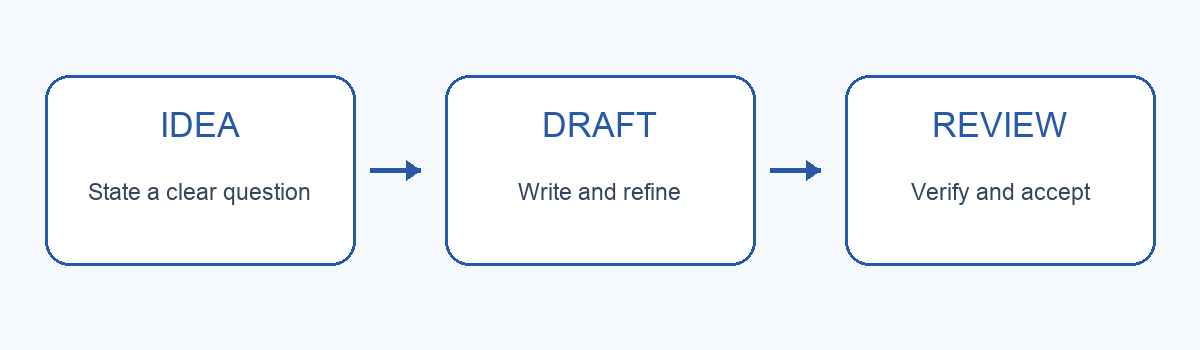
\includegraphics[width=0.93\linewidth]{figures/workflow.png}
\caption{先表达，再推敲，最后确认：人机共写的一个简单循环。}
\label{fig:writing-workflow}
\end{figure}
图~\ref{fig:writing-workflow} 使用项目中的 PNG 图片。可以询问支持视觉的模型：“读取这张图，帮我写一个更准确的中文图注。” 上传自己的图片时，尽量使用简单的英文文件名，并修改 \texttt{includegraphics} 中的路径。

\subsection{参考文献的最小示例}
\texttt{references.bib} 包含一个\textbf{明确标注为教学占位的条目}，可用命令 \verb|\cite{welcome-demo}| 引用，例如这里~\cite{welcome-demo}。项目编译时会生成文末的参考文献列表。

正式写作时，请用你已经核验过的真实文献替换占位条目，并同步更新引用键。不要把教程条目当作真实研究来源。

\section{现在，换成你的主题}
你可以保留这套文件结构，把标题改成自己的题目，再逐步替换正文。遇到编译错误时，先查看日志，定位文件和行号；向 AI 提问时，也可以粘贴相关错误信息，并让它先解释原因。

\begin{center}
\color{ScribeBlue}\large 让工具处理重复工作，把判断留给自己。
\end{center}

\bibliographystyle{plain}
\bibliography{references}
\end{document}
